\TUchapter{Hybrid Extensions}
\TUsection{Introduction}
An objective of this thesis is to make the first known foray into the realm of
attack graphs with real-valued components. This chapter introduces the additional
modeling syntax and generation semantics required to permit real values for
qualities and topologies. Furthermore, some initial attempts at representing
the passage of time are described. 

The ultimate goal of the specification of a hybrid attack graph for cyber
physical systems modeling must be the creation of a formalism capable of
modeling a network containing both traditional information systems (as
existing attack graph incarnations can) and hybrid systems (i.e. those that
can be modeled as hybrid automata). Therefore, the ideal hybrid attack graph
should be able to define systems (assets) that have some equivalence to a
hybrid automaton.

This thesis presents two novel attack graph elements with this requirement
in mind. The first is the ability to give both qualities and topologies
real (continuous domain) values, and correspondingly to permit exploits to
test and operate on these values in the expected ways with a full selection of
real-valued relational and assignment operators. These new types of facts are 
at the heart of this new model. 

The second contribution is modeling the progression
of time; as implemented in this thesis, time progression does not require any
new syntactic elements except those provided in the 
preceding chapter; those syntactic elements, however, are
used in a novel fashion to specify time evolution of facts.

The remainder of this chapter is structured as follows. First, the new
syntactic elements are introduced. Second, the semantic changes that these new
elements impose upon the generation process are described. Then the
convention for the specification of time evolution is described. 
Finally, a pair of examples is provided.
\TUsection{Definition of New Syntax}
\TUsubsection{Terminology}
First and foremost, a discussion of the new terminology involved in the
transition to hybrid attack graphs is required. This is mostly concerned with
facts, as the transition to hybrid attack graphs is consists mostly of changes
to the fact system.

Until now, qualities have had only string type values, and
topologies have had no values at all. In this chapter, that changes. Although
there will always remain a need for these discrete valued qualities and name
only topologies, there is also a need for qualities with 
continuous, numerical values. The introduction of a second type of quality
value is somewhat less jarring, however, than that of topologies with
values.

As the hybrid attack graph introduced by this thesis is a strict superset
of the University of Tulsa style discrete attack graph, the existing style
of quality and topology facts remains valid in the new language and therefore
must be distinguished from the new type of fact in some way. The discrete
only facts, therefore, are called \emph{token valued} (or \emph{token facts}),
whereas the new continuous facts are called \emph{real valued} (or \emph{real
facts}).

% Additionally, later in this chapter another class of fact is introduced: a
% rate fact, which is a special case of a real fact. Rate facts are not a new
% syntactic element but are rather specified by convention and invoked by the
% new timing capability. TODO: this isn't true; add to future work.
\TUsubsection{Operators}
At the heart of the hybrid attack graph lies the new real facts. Their
existence marks the introduction of a true type system to the attack graph
model, which must be dealt with in some fashion. Furthermore, these new real 
facts demand new real operators to deal with them.

Typing is dealt with by ensuring that the sets of both assignment and relational
operators used for token and real facts are disjoint. While token qualities are
assigned with the \texttt{=} operator, real facts (both quality and topology)
are assigned using a \texttt{:=} operator.

As for the relational operators, token facts are tested using \texttt{=} 
and \texttt{!=}. The relational operators permitted for real facts (both
quality and topology) are different: \texttt{==}, \texttt{>}, \texttt{>=},
\texttt{<=}, and \texttt{<>} (for not equal).

Finally, because a principal property of real values is their suitability for
arithmetic, a number of new operators are introduced for use in exploit
postconditions only, with their straightforward C-like meanings: \texttt{:=},
\texttt{+=}, \texttt{-=}, \texttt{*=}, and \texttt{/=}. Note that currently
these operators take only literal reals as their second operand; variables
are not permitted.
\TUsubsection{Topology values}
Due to the usefulness of permitting real valued relationships between assets,
be they physical such as distance, or IT related like latency or signal
strength, in hybrid attack graphs, real topologies may take values. The
syntax for this is identical to the existing token topology syntax, except
followed by an operator and a number.

\TUsubsection{The update operation}
Because of the semantics of binary arithmetic operators such as \texttt{+=},
the term \texttt{insert} in postcondition operations is somewhat psychologically
unsatisfactory. Therefore, it is now aliased to \texttt{update}, a semantically
identical operation. In spite of its apparent redundancy, it provides for
future expansion as well as readability.
\TUsection{Time}
A fundamental requirement of modeling hybrid systems is the progression of
time, as the most interesting and distinctive properties of physical processes
are their evolution over time. Another goal is to avoid introducing additional
special cases. To that end, this section introduces a method for handling time
using only previously introduced attack graph functionality.
\TUsubsection{Time exploits}
Exploits are not just for adversary actions in hybrid attack graphs. Time is 
implemented using
a single group of global exploits, each of which increments a class of assets'
position in time depending upon its particular state. Their globalness
triggers on all assets simultaneously, while the grouping causes
all the time exploits to trigger in concert. As before,
an important requirement is that the sets of facts affected by time exploits
be disjoint over all grouped time exploits to avoid indeterminate behavior.

A selection of time exploits is provided in Fig.~\ref{fig:illustrative_time_xp}
that might, when paired with the network model in 
Fig.~\ref{fig:illustrative_time_nm}, simplistically model
a car driving away from a wall unless somehow compromised by an attacker,
who causes the car to drive toward the wall at a constant rate.

\begin{figure}
\begin{lstlisting}
network model=
    assets:
        civic;
        wall;
    facts:
        platform:civic,cpe:/h:honda:civic;
        quality:civic,compromised=true;
        quality:civic,status=up;

        platform:wall,cpe:/h::wall;

        topology:civic<->wall,distance:=50;
.
\end{lstlisting}
\caption{Car example network model}
\label{fig:illustrative_time_nm}
\end{figure}

\begin{figure}
\begin{lstlisting}
global group(time) exploit car_depart(c,w)=
    preconditions:
        platform:c,cpe:/h:honda;
        quality:c,compromised != true;
        platform:w,cpe:/h::wall;
        quality:c,status=up;
    postconditions:
        update topology:c<->w,distance+=25;
.

global group(time) exploit car_approach(c,w)=
    preconditions:
        platform:c,cpe:/h:honda;
        quality:c,compromised=true;
        platform:w,cpe:/h::wall;
        quality:c,status=up;
        topology:c<->w,distance>25;
    postconditions:
        update topology:c<->w,distance-=25;
.

global group(time) exploit car_crash(c,w)=
    preconditions:
        platform:c,cpe:/h:honda;
        quality:c,compromised=true;
        platform:w,cpe:/h::wall;
        quality:c,status=up;
        topology:c<->w,distance<=25;
    postconditions:
        update topology:c<->w,distance:=0;
        update quality:c,status=down;
.
\end{lstlisting}
\caption{Car example exploit patterns (note time)}
\label{fig:illustrative_time_xp}
\end{figure}

This method of modeling time requires time to be quantized and time stepping
behavior to be used. 

\TUsection{Generation process changes}
\TUsubsection{Topologies}
Even without concern for real types, the move to hybrid attack graphs 
introduces a new, more basic requirement for the processing of preconditions
and postconditions: topology values. The topology fact handling is updated
to be virtually identical to the handling of qualities. In fact, in the hybrid 
attack graph
reference implementation, every topology, even token topologies, has a value:
real topologies have floating-point values, and token topologies have boolean
values.

This results in the new factbase data structure provided in 
Fig.~\ref{fig:netstate_map_hybrid_pc}. The intermediate hash map representation
for topology facts is keyed on source asset names, with values that are
themselves hash maps keyed on destination asset names, with values that are
\emph{also} hash maps keyed on topology names, with values storing topology
values. Again, for token topologies, this value is always the boolean true.

\begin{figure}
\begin{lstlisting}
fact-tuple = ('quality', asset, name, value) or
           = ('topology', source, dest, name) or
           = ('platform', platform_part, ..., language)

type network_state:
    assets : set of strings;
    factbase : set of fact-tuples;
    qualities : map (keys=assets, 
                     vals=map(keys=quality_name,
                              vals=quality_value))
    topologies : map (keys=src_assets, 
                      vals=map(keys=dest_asset,
                               vals=map(keys=topology,
                                        vals=values))
\end{lstlisting}
\caption{Updated hybrid network state datatype pseudocode}
\label{fig:netstate_map_hybrid_pc}
\end{figure}
\TUsubsection{Matching}
With the introduction of new relational operators, more advanced
precondition processing is required. Happily, the changes introduced
in the previous chapter anticipated this, so the heavy lifting required for
fact value lookup already exists. All that remains is the mapping of the
parsed attack graph operators onto implementation operators in the generation
software.

As illustrated in the pseudocode in Fig.~\ref{fig:hybrid-matching}, this is
done in the reference implementation by maintaining a map from the string
representations of the relational operators onto (pointers to) boolean 
functions that apply
them. The new relational operator precondition processing does not impact the
remainder of the generation process.

\begin{figure}
\begin{lstlisting}
RELOPS = map(keys = ('==', '<>', '>=', '<=',
                     '<', '>', '=', '!='),
             vals = (associated functions))
             
def matches_topology(source, dest, name, value=True, 
                     op='==', check_reverse=False):
    if source in factbase.topologies and
      dest in factbase.topologies[source] and
      name in factbase.topologies[source][dest]:
        my_value = factbase.topologies[source][dest][name]
    else:
        return False

    if type(my_value) != type(value):
        Error: Cannot match token values with real values.
    
    if check_reverse:
        return RELOPS[op](my_value, value) and
               matches_topology(dest, source, name, 
                                value=value, op=op)
    else:
        return RELOPS[op](my_value, value)

def matches_quality(asset, name, value, op='=='):
    if asset in factbase.qualities and
      name in factbase.qualities[asset]:
        my_value = factbase.qualities[asset][name]
    else:
        return False
    
    if type(my_value) != type(value):
        Error: Cannot match token values with real values.
    
    return RELOPS[op](my_value, value)
\end{lstlisting}
\caption{Hybrid precondition matching pseudocode}
\label{fig:hybrid-matching}
\end{figure}
\TUsubsection{Updating}
The hybrid attack graph includes assignment operators that require new
postcondition handling that closely parallels their precondition handling.
The same issues are addressed here; value querying and setting is already
handled, but operator selection is not. The pseudocode for this process is
presented in Fig.~\ref{fig:hybrid-postcondition}.

\begin{figure}
\begin{lstlisting}
ASSIGNOPS = map(keys=('+=', '-=', '*=','/=', ':=', '='),
                vals=(associated functions)

def set_quality(factbase, asset, name, value, op='='):
    if asset in factbase.qualities and
      name in factbase.qualities[asset]:
        my_value = factbase.qualities[asset][name]
    else:
        my_value = 0
    new_value = ASSIGNOPS[op](my_value, value)
    update factbase with:
        factbase.qualities[asset][name] = new_value

def set_topology(factbase, source, dest, name, 
                 value=True, op=None):
    if not op: # Token
        update factbase with:
            factbase.topologies[source][dest][name] = value
    else: # Real
        if source in factbase.topologies and
          dest in factbase.topologies[source] and
          name in factbase.topologies[source][dest]:
            my_value = self.assets[source].get_topology(
                dest, name
              )
        else:
            my_value = 0
        new_value = ASSIGNOPS[op](my_value, new_value)
        update factbase with:
        factbase.qualities[source][dest][name] = new_value
\end{lstlisting}
\caption{Hybrid postcondition application pseudocode}
\label{fig:hybrid-postcondition}
\end{figure}
\TUsection{Examples}
\TUsubsection{Car}
A useful preliminary example is the scenario involving a car as described in
Figs.~\ref{fig:illustrative_time_xp} and \ref{fig:illustrative_time_nm}. The
corresponding attack graph for that scenario is given in 
Fig.~\ref{fig:fullbunny_simple_ag}. As the car is compromised from the start,
it only has three states. Note the exploit transitions,
both of which are collected into a group called ``time'', signifying that
they represent time steps. The global and grouping mechanisms, however, only 
truly become dramatic once combined with discrete exploits causing mode
transitions, and even more so once multiple assets are involved.
\label{sec:car}

\begin{figure}
\centering
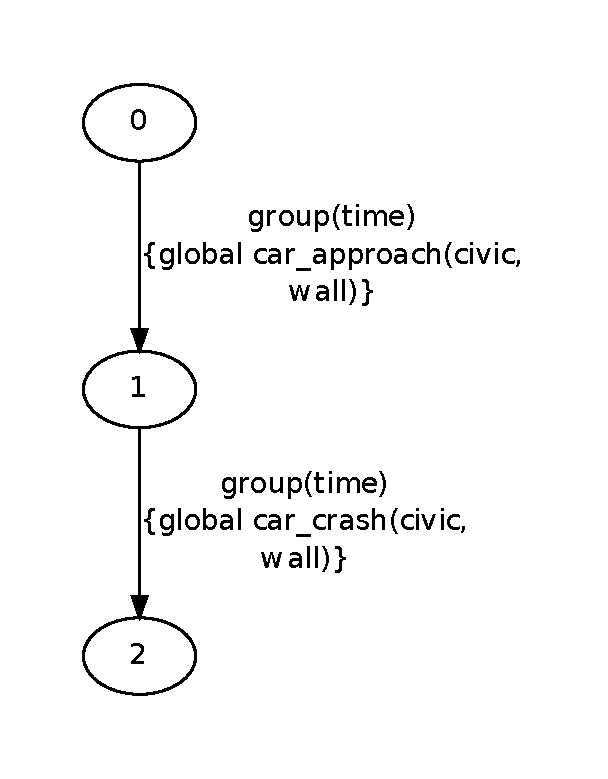
\includegraphics[height=3in]{ag_car/simple/full_bunny_1_ag_5}
\caption{Simple car attack graph}
\label{fig:fullbunny_simple_ag}
\end{figure}

Suppose the initial conditions were changed so that the \texttt{compromised}
quality began as \texttt{false}, and an additional exploit called \texttt{own_civic}
were added so as to match the patterns given in Fig.~\ref{fig:fullbunny_one_xp}.

\begin{figure}
\begin{lstlisting}
global group(time) exploit car_depart(c,w)=
    preconditions:
        platform:c,cpe:/h:honda;
        quality:c,compromised != true;
        platform:w,cpe:/h::wall;
        quality:c,status=up;
    postconditions:
        update topology:c<->w,distance+=25;
.

global group(time) exploit car_approach(c,w)=
    preconditions:
        platform:c,cpe:/h:honda;
        quality:c,compromised=true;
        platform:w,cpe:/h::wall;
        quality:c,status=up;
        topology:c<->w,distance>25;
    postconditions:
        update topology:c<->w,distance-=25;
.

global group(time) exploit car_crash(c,w)=
    preconditions:
        platform:c,cpe:/h:honda;
        quality:c,compromised=true;
        platform:w,cpe:/h::wall;
        quality:c,status=up;
        topology:c<->w,distance<=25;
    postconditions:
        update topology:c<->w,distance:=0;
        update quality:c,status=down;
.

exploit own_civic(c)=
    preconditions:
        platform:c,cpe:/h:honda:civic;
        quality:c,compromised=false;
        quality:c,status=up;
    postconditions:
        update quality:c,compromised=true;
.
\end{lstlisting}
\caption{One-car hybrid example}
\label{fig:fullbunny_one_xp}
\end{figure}

In this case, the resulting attack graph (shown in 
Fig.~\ref{fig:fullbunny_one_ag} to a maximum generation depth of 5) clearly
illustrates the interaction of the discrete behavior of the attacker (an
attack occuring in the ``cyber'' world) with the continuous evolution of the
car (in the physical world). This embodies a common trait of hybrid systems
and also hybrid attacks: their discrete behavior acts to place them into
operational modes wherein the passage of time causes important behavior. In
this case, the evolution of time is clearly denoted by the transitions labeled
\texttt{group(time)}.

\begin{figure}
\centering
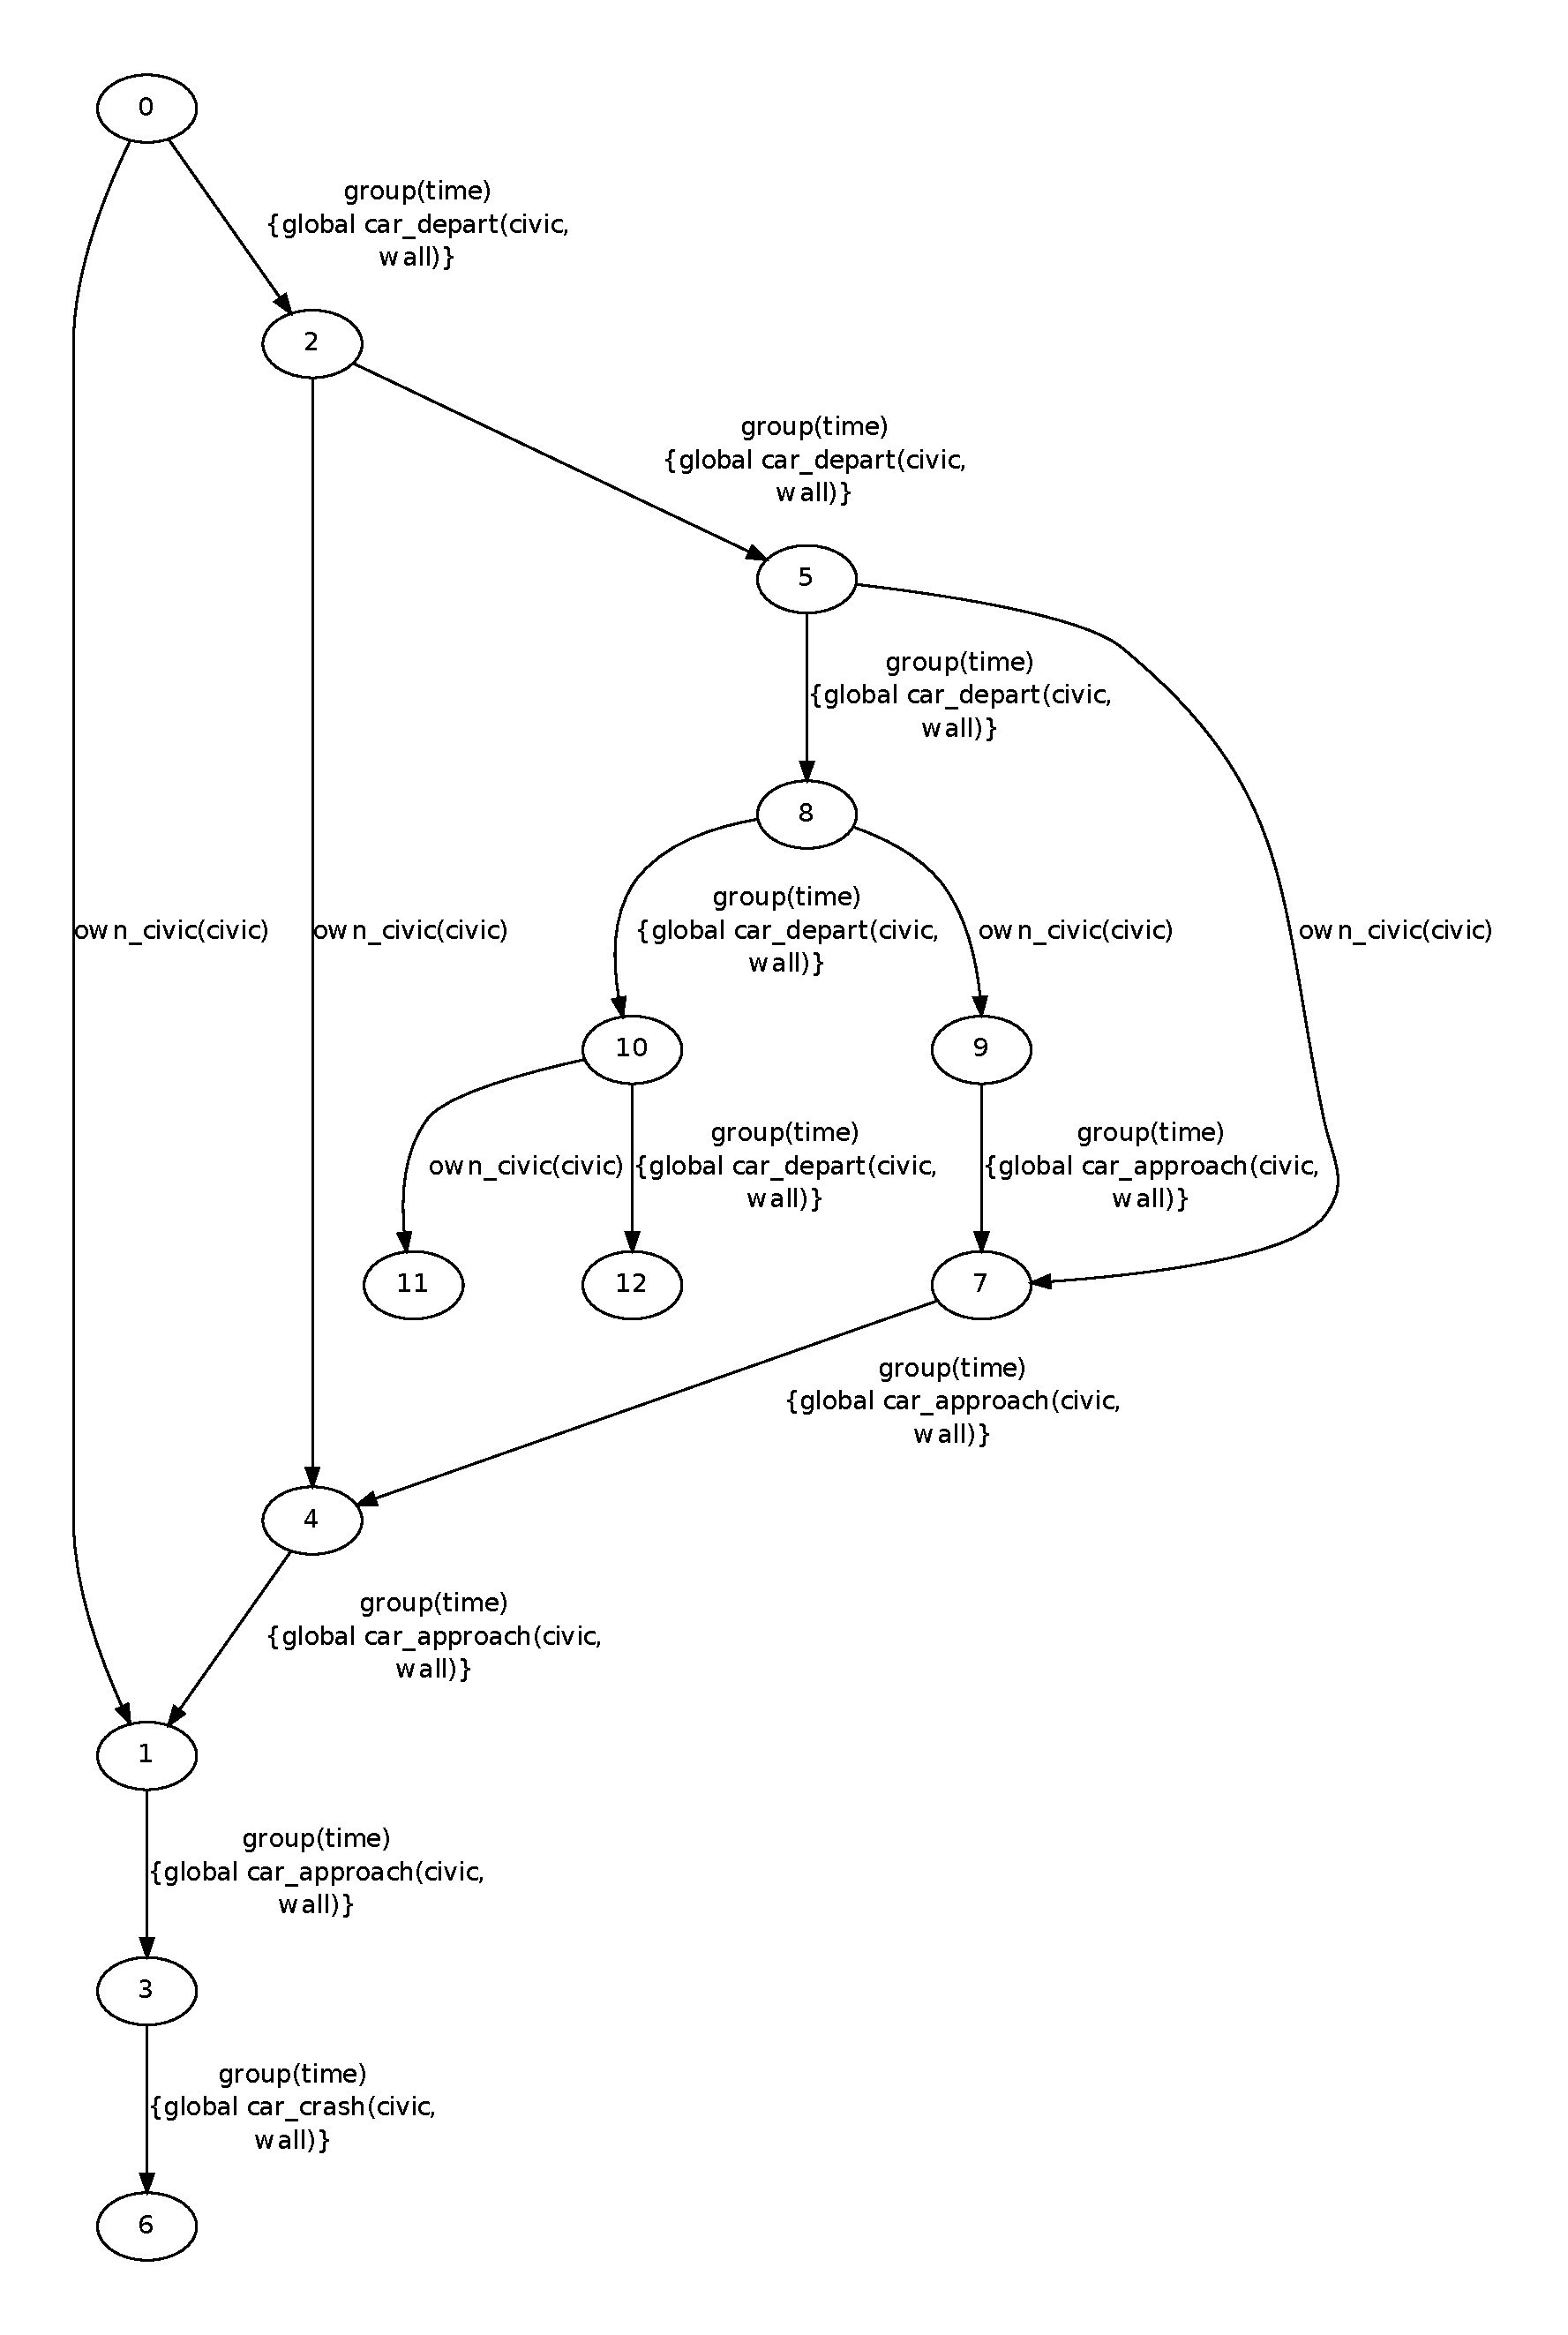
\includegraphics[height=0.9\textheight]{ag_car/onecar/full_bunny_onecar_ag_5}
\caption{One-car automotive attack graph}
\label{fig:fullbunny_one_ag}
\end{figure}

One final automobile example serves to illustrate the behavior of the
combined global and grouped exploits and their use in implementing
timing behavior. Consider the case that, while keeping the exploits
as in Fig.~\ref{fig:fullbunny_one_xp}, introduces an additional car
that drives away from the wall
at the same rate as \texttt{civic} but is \emph{not} vulnerable to the 
\texttt{own_civic} exploit. This network model is provided in 
Fig.~\ref{fig:fullbunny_two_nm}.

\begin{figure}
\begin{lstlisting}
network model=
    assets:
        civic;
        accord;
        wall;
    facts:
        platform:civic,cpe:/h:honda:civic;
        quality:civic,compromised=false;
        quality:civic,status=up;
        
        platform:accord,cpe:/h:honda:accord;
        quality:accord,compromised=false;
        quality:accord,status=up;

        platform:wall,cpe:/h::wall;

        topology:civic<->wall,distance:=50;
        topology:accord<->wall,distance:=60;
.
\end{lstlisting}
\caption{Two-car example network model}
\label{fig:fullbunny_two_nm}
\end{figure}

The resulting attack graph is provided in Fig.~\ref{fig:fullbunny_two_ag}.
Observe the sometimes heterogeneity of the time evolution exploit groups.
Of particular interest is the transition from state 3 to state 6, in which
the crashing of the Civic has the discrete consequence of placing it into a
mode in which it no longer changes state with time.

\begin{figure}
\centering
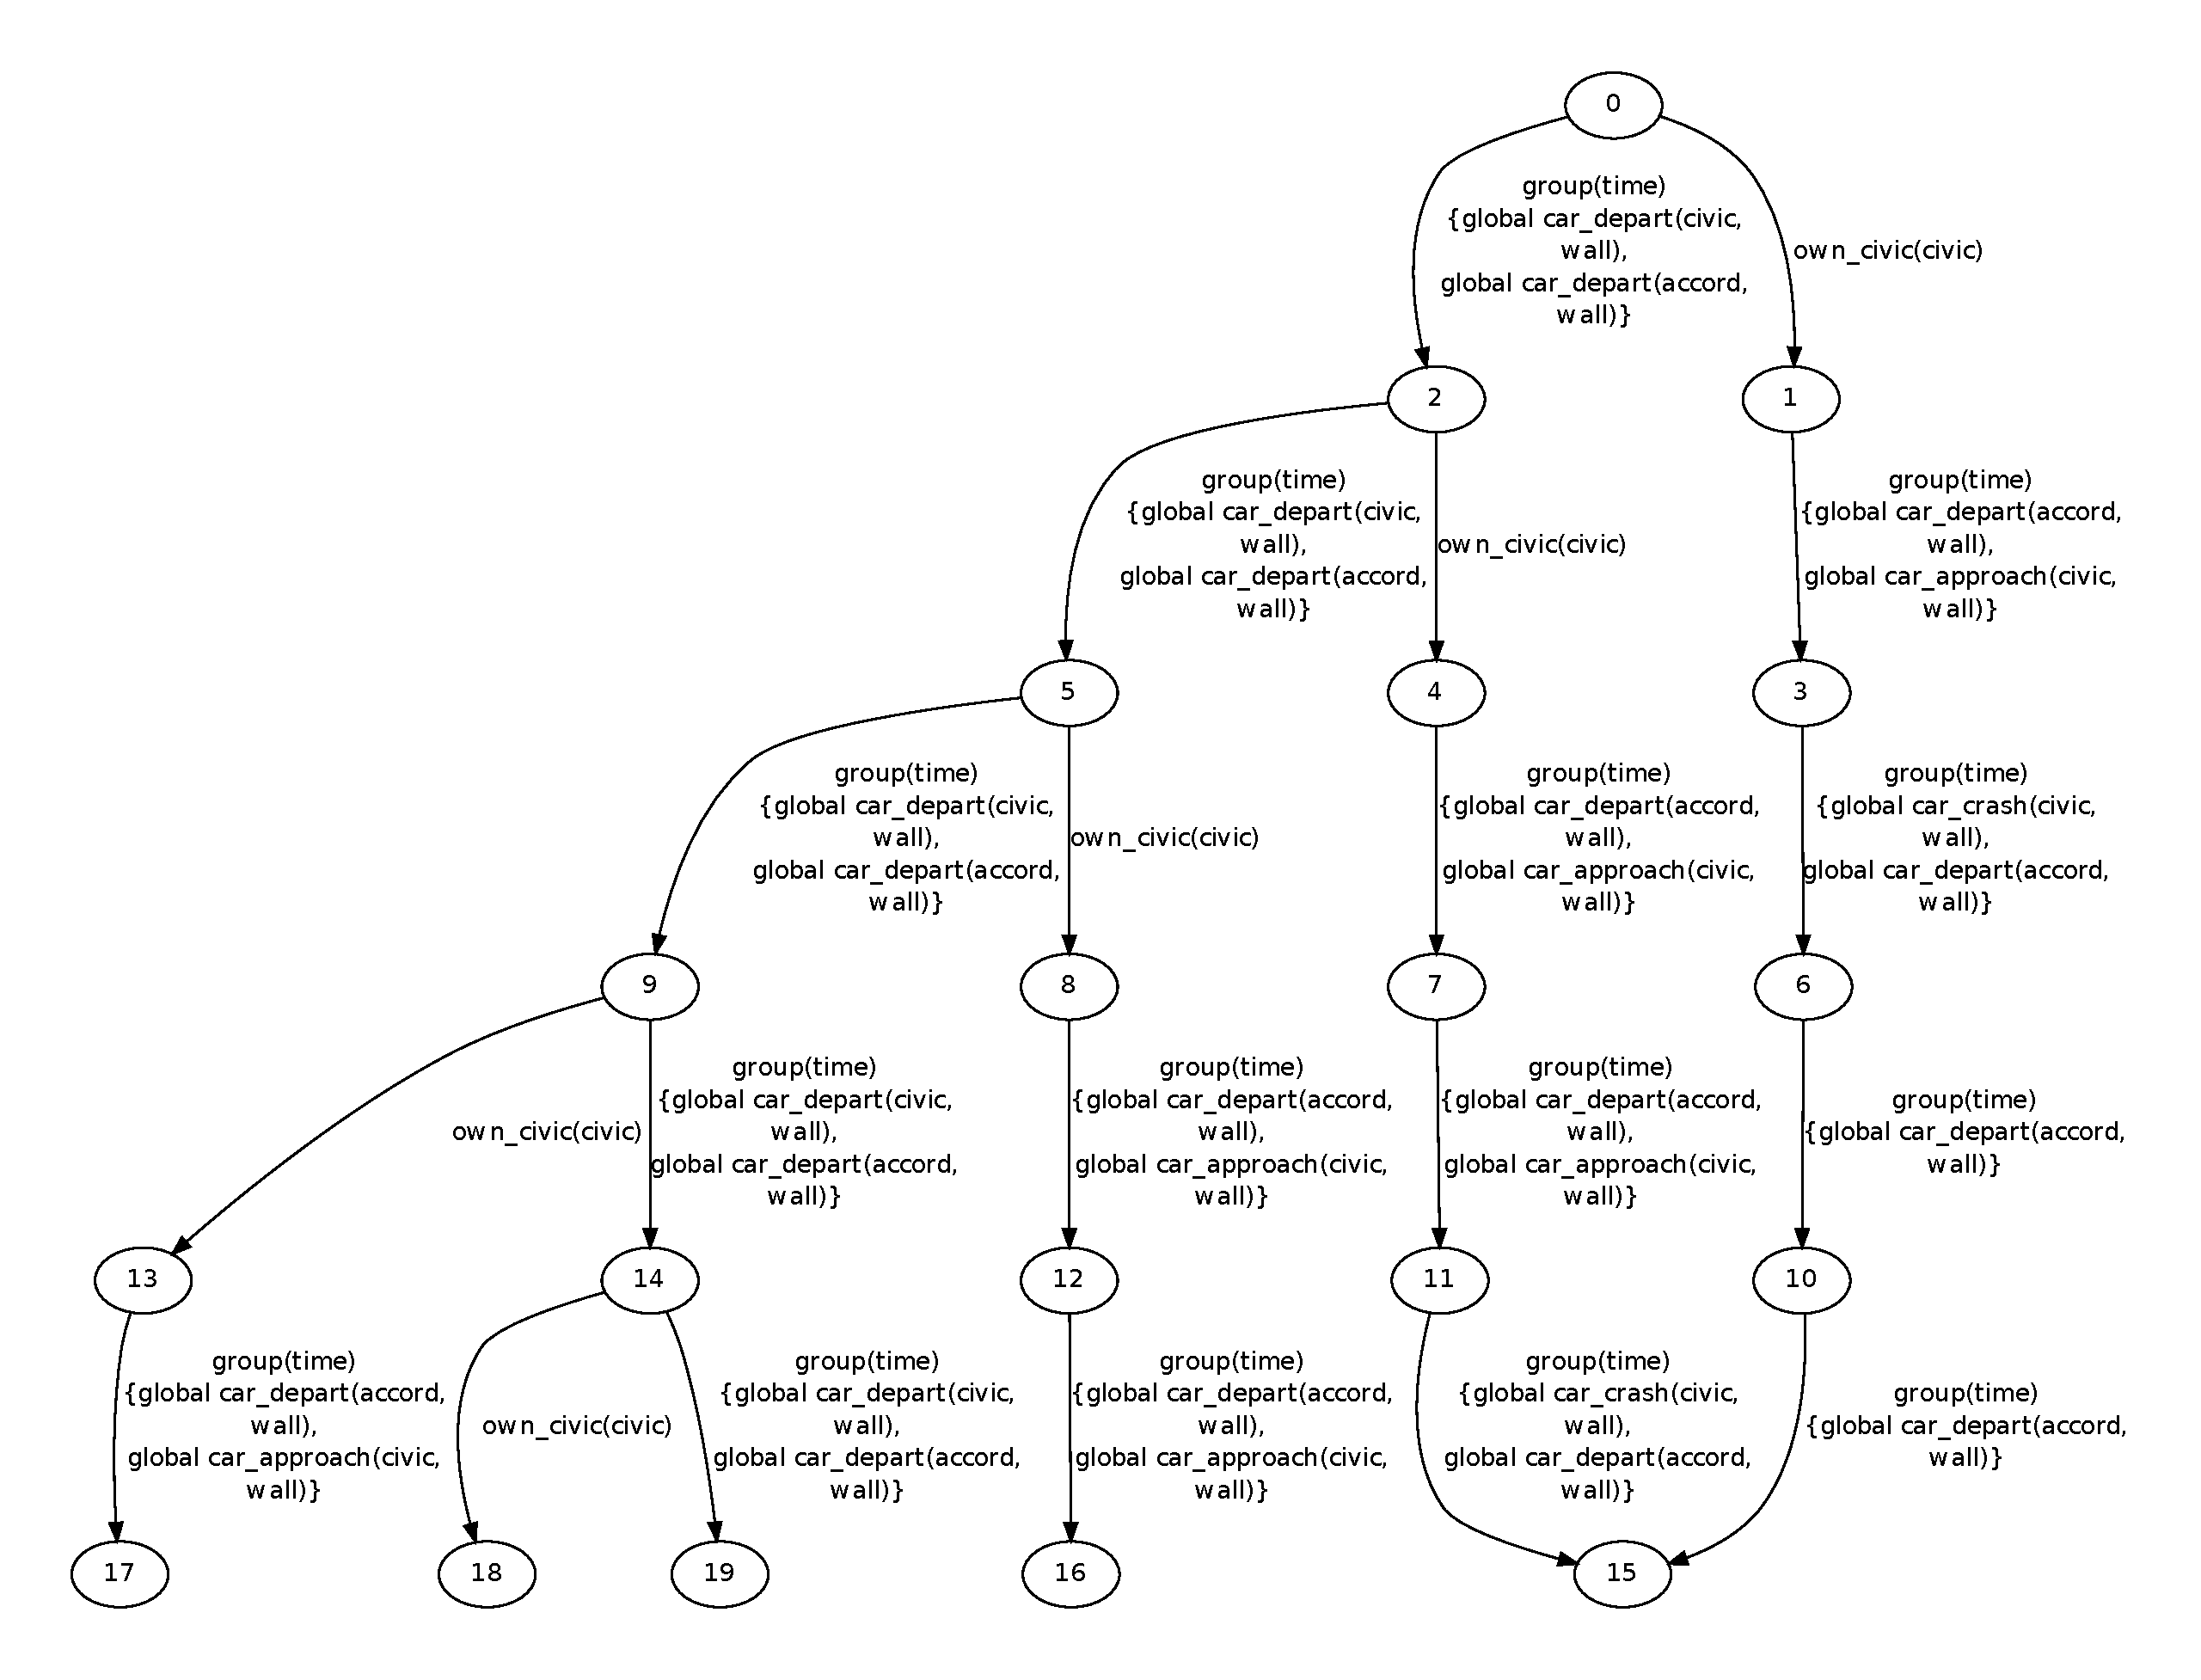
\includegraphics[angle=90,width=0.9\textwidth]{ag_car/twocar/full_bunny_twocar_ag_5}
\caption{Two-car automotive attack graph}
\label{fig:fullbunny_two_ag}
\end{figure}
\TUsubsection{Denial of Sleep}
\label{sec:rfid}
The final example serves to demonstrate further the interaction of discrete
attacks with time; it is also used later to discuss scaling behavior. The network
model given in Fig.~\ref{fig:rfid1_nm} describes a system of a single
RFID reader with a single RFID tag, in the ISO 18000-7 system as described 
in Section~\ref{sec:bg:rfid}. The tag begins with a battery life of 100, which
is drained at a rate of 25 per time step if the sleep denial attack is being
executed, and at a rate of 10 per time step if not. This behavior is shown in
the exploit patterns in Fig.~\ref{fig:rfid1_real_xp}. The scenario's discrete
attacks \texttt{own\_reader} (which gives the attacker control of
the reader) and \texttt{deny\_sleep} (which causes a tag to enter the
denial of sleep mode) are shown in Fig.~\ref{fig:rfid1_token_xp}.

\begin{figure}
\begin{lstlisting}
network model = 
    assets :
        attacker;
        reader;
        tag0;
    
    facts :
        # Reader:
        platform:reader,cpe:/h::VulnerableReader;
        quality:reader,status=up;
        
        # Tag:
        platform:tag0,cpe:/h::Tag;
        quality:tag0,status=up;
        quality:tag0,power:=100;
        quality:tag0,mode=sleep;
        
        # Topologies:
        topology:attacker -> reader,connected_network;
        topology:reader -> tag0,connected_rfid;
.
\end{lstlisting}
\caption{One tag RFID system network model}
\label{fig:rfid1_nm}
\end{figure}

\begin{figure}
\begin{lstlisting}
global group(time) exploit wake_power_dec(t)=
    preconditions:
        platform:t,cpe:/h::Tag;
        quality:t,status=up;
        quality:t,mode=wake;
        quality:t,power>25;
    postconditions:
        update quality:t,power-=25;
.

global group(time) exploit sleep_power_dec(t)=
    preconditions:
        platform:t,cpe:/h::Tag;
        quality:t,mode=sleep;
        quality:t,status=up;
        quality:t,power>10;
    postconditions:
        update quality:t,power-=10;
.

global group(time) exploit wake_power_die(t)=
    preconditions:
        platform:t,cpe:/h::Tag;
        quality:t,mode=wake;
        quality:t,status=up;
        quality:t,power<=25;
    postconditions:
        update quality:t,power:=0;
        update quality:t,status=down;
.

global group(time) exploit sleep_power_die(t)=
    preconditions:
        platform:t,cpe:/h::Tag;
        quality:t,mode=sleep;
        quality:t,status=up;
        quality:t,power<=10;
    postconditions:
        update quality:t,power:=0;
        update quality:t,status=down;
.
\end{lstlisting}
\caption{One tag RFID system continuous exploit patterns}
\label{fig:rfid1_real_xp}
\end{figure}

\begin{figure}
\begin{lstlisting}
exploit own_reader(a, r)=
    preconditions:
        platform:r,cpe:/h::VulnerableReader;
        quality:r,status=up;
        topology:a->r,connected_network;
    postconditions:
        insert topology:a->r,access_admin;
.

exploit deny_sleep(a, r, t)=
    preconditions:
        platform:r,cpe:/h::VulnerableReader;
        quality:r,status=up;
        
        platform:t,cpe:/h::Tag;
        quality:t,status=up;
        quality:t,mode=sleep;
        
        topology:a->r,access_admin;
        topology:r->t,connected_rfid;
    postconditions:
        update quality:t,mode=wake;
.
\end{lstlisting}
\caption{One tag RFID system discrete exploit patterns}
\label{fig:rfid1_token_xp}
\end{figure}

Two attack graphs help to demonstrate the execution of this model. The first is
given in Fig.~\ref{fig:rfid1_ag6}, which is the attack graph generated to a
depth of 6. Observe that the leftmost set of edges is the worst case
scenario: the attacker immediately takes control of the network and kills
the tags in only 4 timesteps. The rightmost edge, then, is the best case
scenario: in this situation, the attacker never (to a
depth of 6) acts. The only transitions are those caused by the normal
time evolution of the system.

Likewise, Fig.~\ref{fig:rfid1_ag11} is the attack graph generated to its
full depth. There are only two leaf nodes: state 21, in which the attacker
has executed the denial of sleep attack to the demise of the tag, and state
40, in which the tag has died on its own.

\begin{figure}
\centering
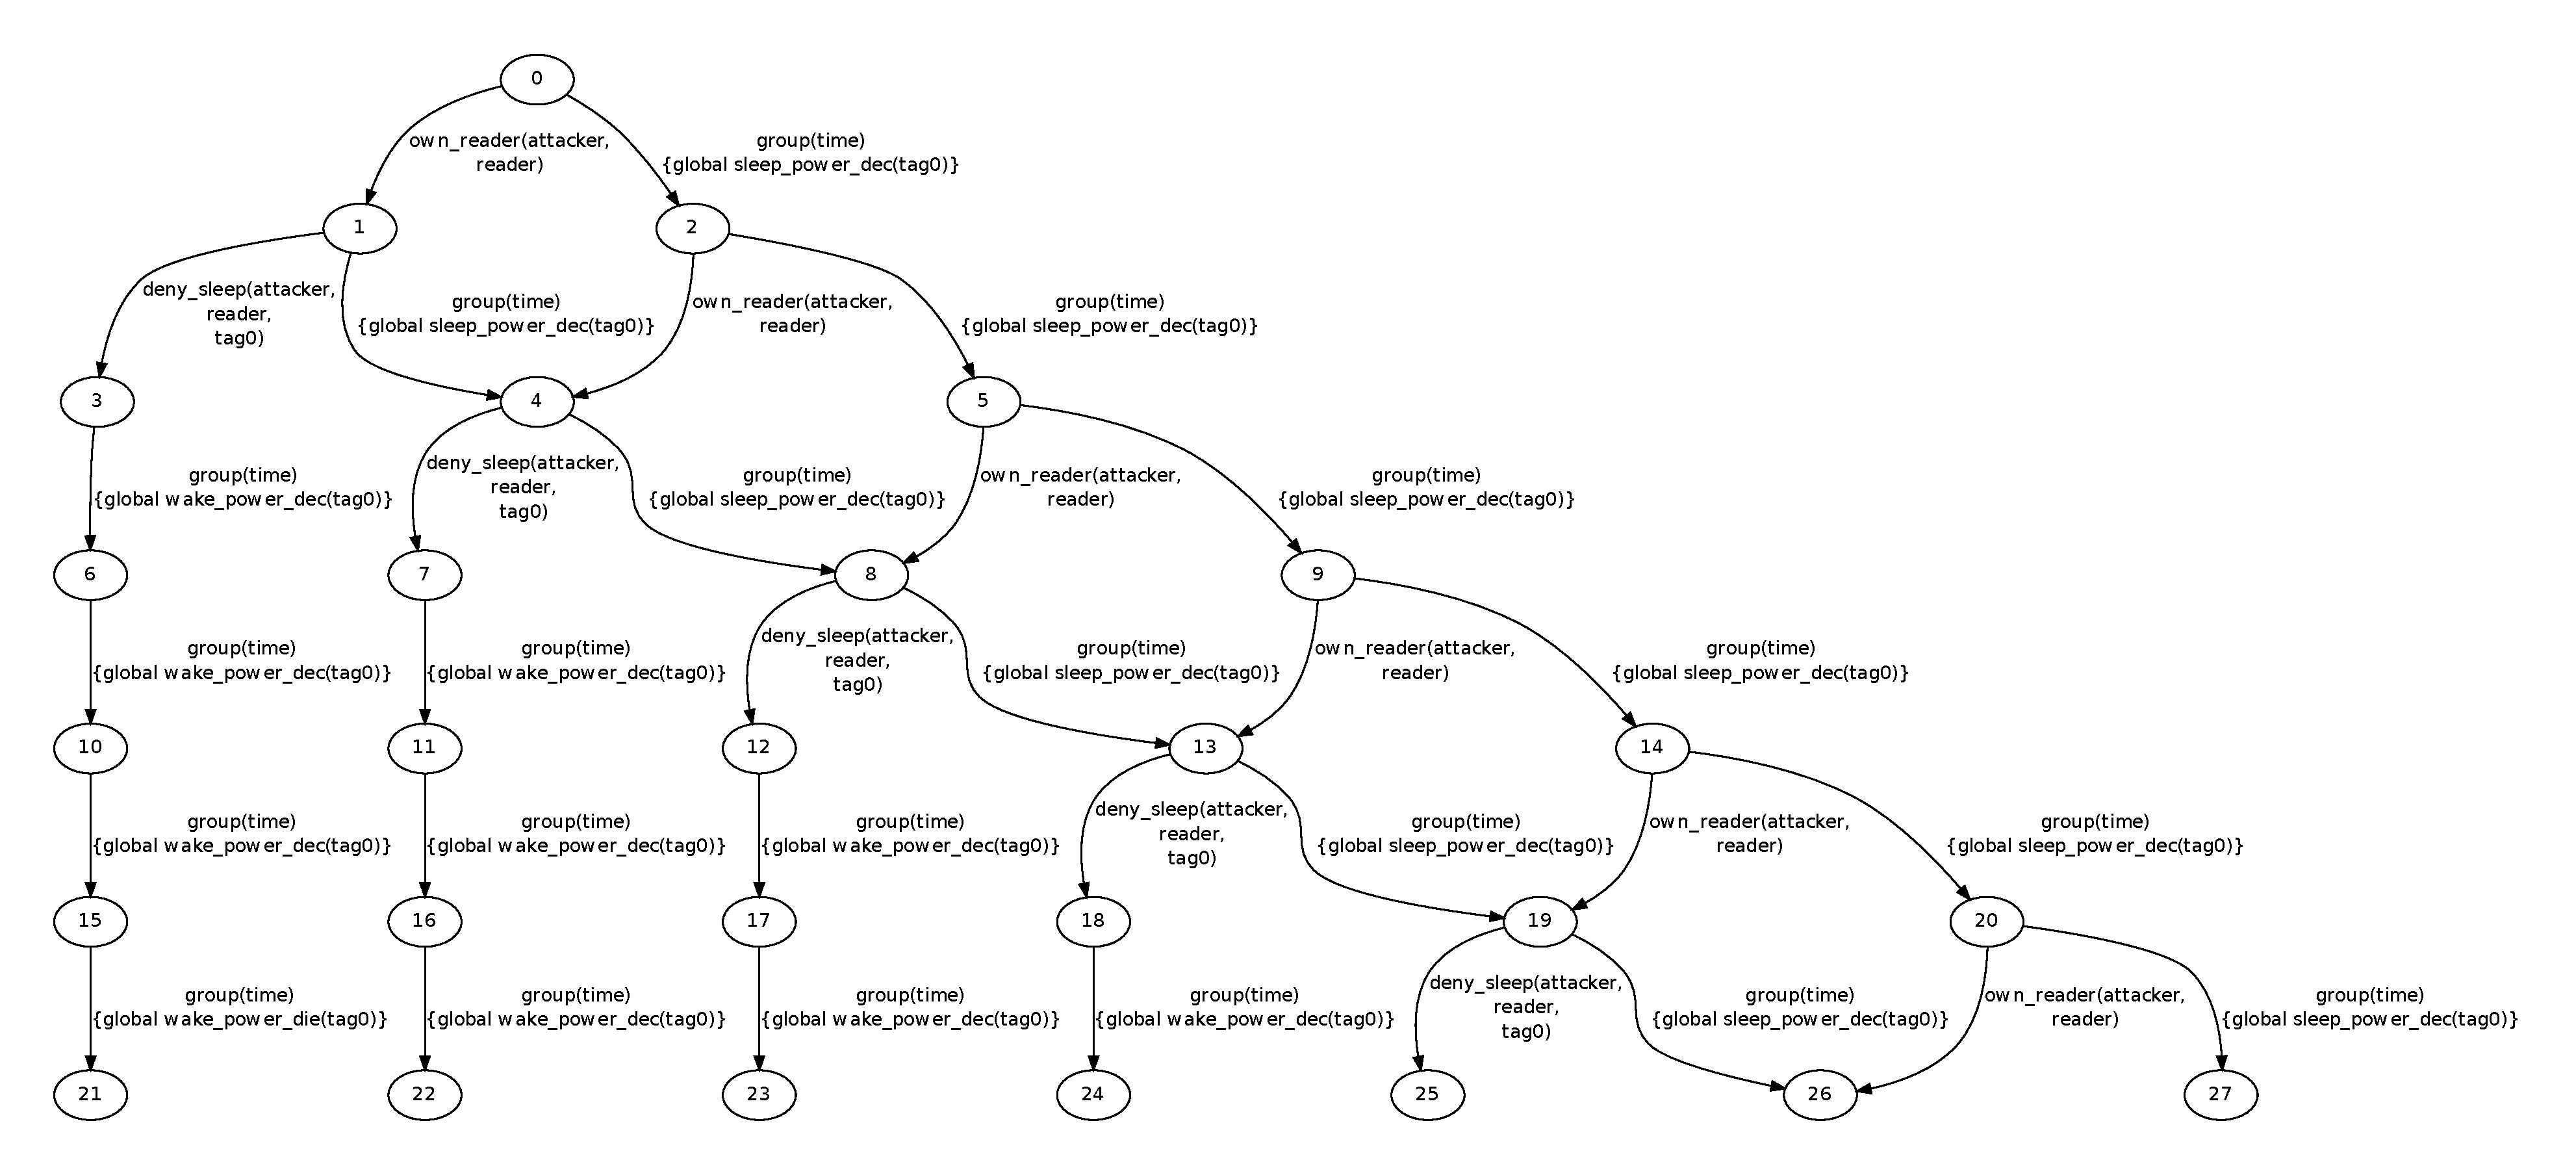
\includegraphics[angle=90,height=0.9\textheight]{ag_dash7/sleep_ag_6}
\caption{One tag RFID system attack graph (depth of 6)}
\label{fig:rfid1_ag6}
\end{figure}

\begin{figure}
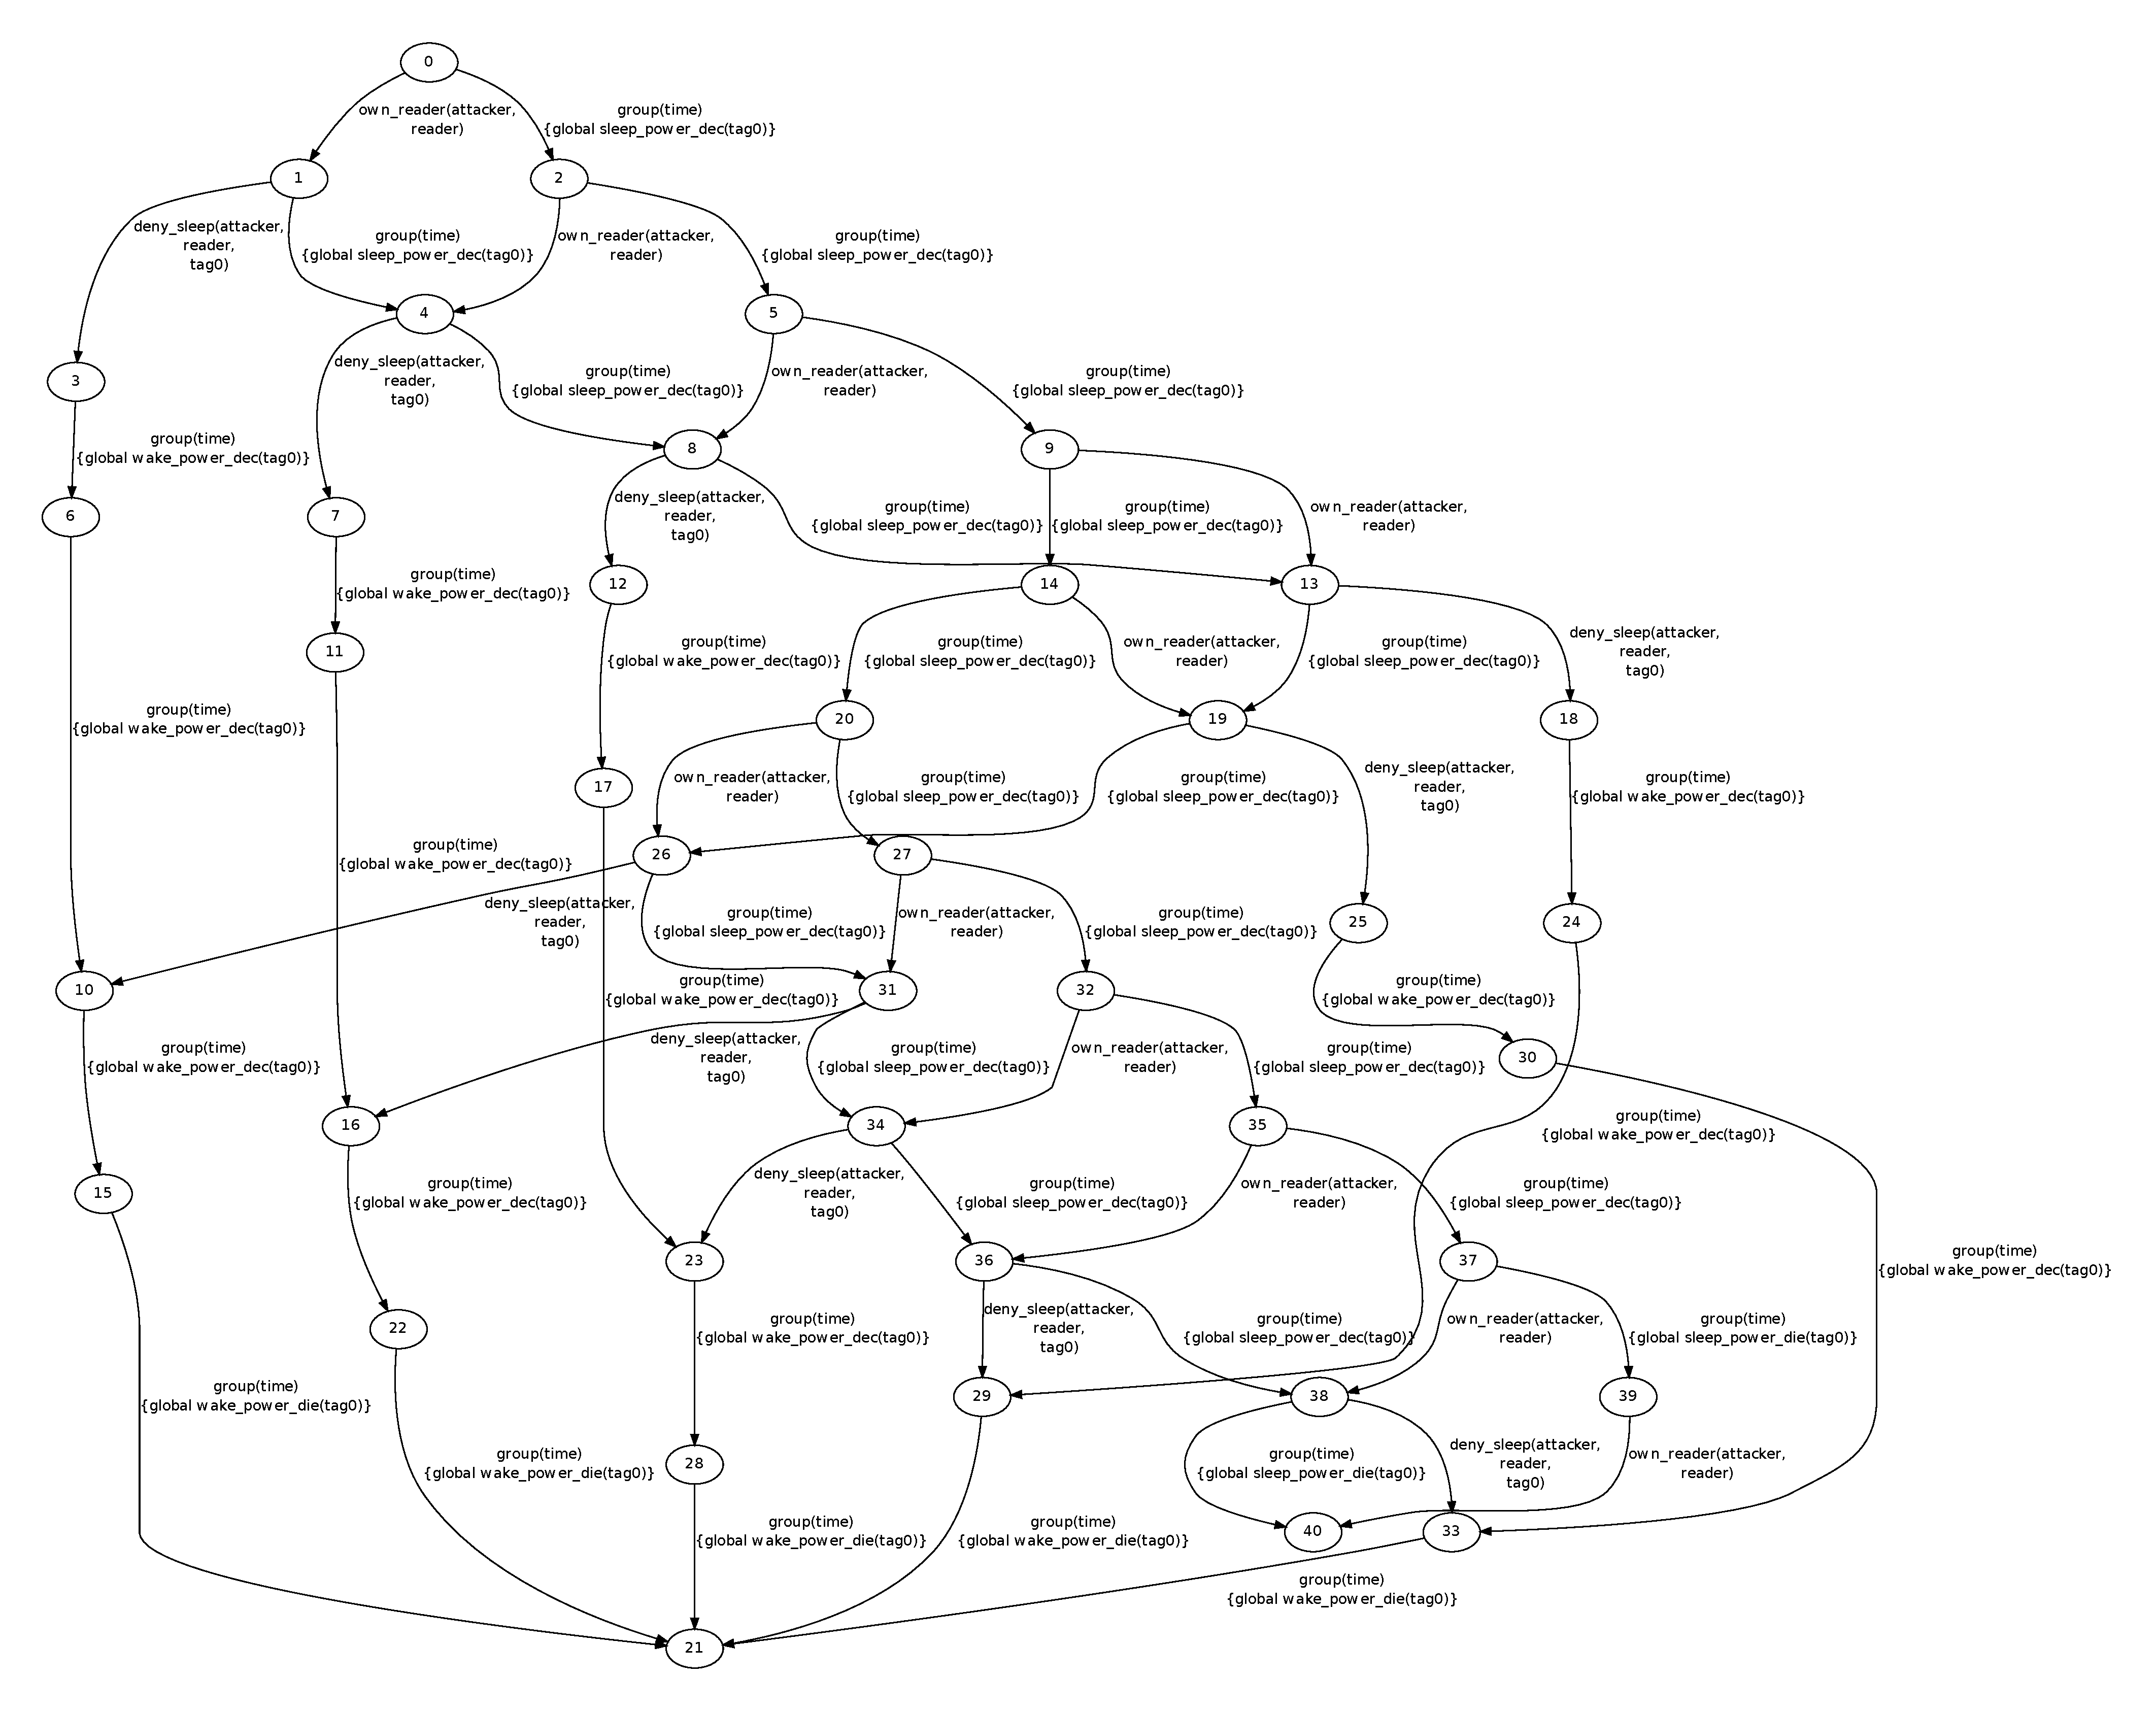
\includegraphics[width=\textwidth]{ag_dash7/sleep_ag_11}
\caption{One tag RFID system attack graph (full depth)}
\label{fig:rfid1_ag11}
\end{figure}